% 1. novel approach, why? protection goals and performance → security and efficiency
% 2. what precisely was done at the TUD chair → say that their research proved the potential of NC and that's why we persue it here again
% 3. NC provides no confidentiality/integrity guarantees → we implement encryption+authentication
% 3.1 Availability only partially adressed
% 3.2 recall NoC architecture → this is implemented in the network interfaces
% 4. Different variants envisioned (3 methods) + comparison with uncoded variant where applicable
% 5. Multiple paths focus → why multiple paths in the first place? → chance to avoid compromised routers, still have enough flits
%    thanks to NC
% 6. Routing strategies: deterministic vs. non-deterministic routing → XY, smart random XY, ROMM+XY, ROMM+srXY
% 7. Attacker/Threat model
% 8. Evaluation
% Always refer to the chapters that explain this in detail
In this thesis, a novel approach for securing the communications in a \gls{noc} is pursued. In Section \ref{sec:nocsecurity}, it was shown that
attacks specifically tailored for \gls{noc} architectures are feasible and practical. In particular, hardware trojans pose a potent threat to
\glspl{mpsoc} employing \glspl{noc}.

The security measures that are explored in this work aim to provide confidentiality and integrity to communications passing through a \gls{noc}. To
achieve this, a new network interface design is proposed. Since all flits that enter the \gls{noc} must pass through a network interface, this is the
ideal location to implement cryptographic protection. In the proposed design, it encrypts all outgoing flits, which can only be decrypted by the
receiver. In addition, a \gls{mac} is computed that is sent together with the encrypted flits. On the receiver side, the flits are decrypted and the
\gls{mac} is verified. This scheme is visualized in Figure \vref{fig:nocflitencauth} and further explained in Section (insert ref here).

\begin{figure}
    \centering
    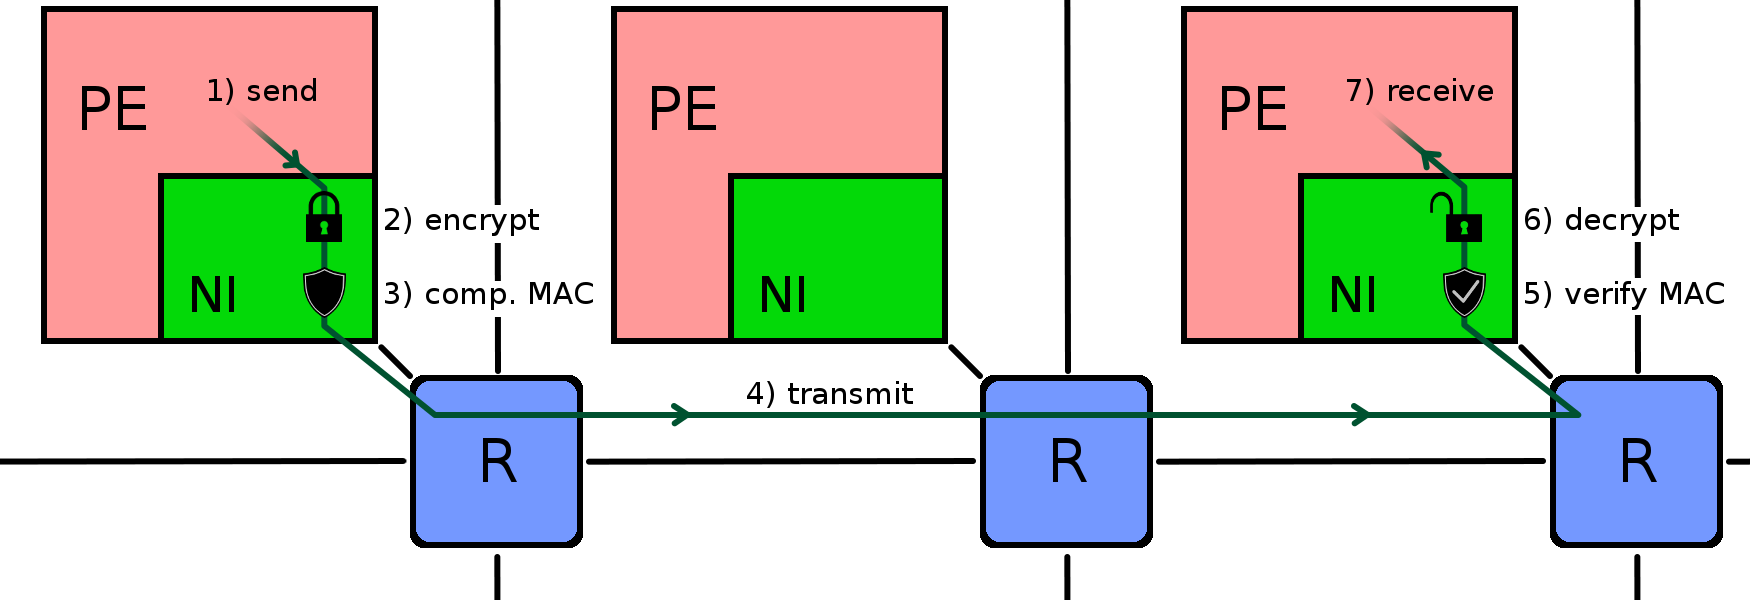
\includegraphics[width=\textwidth]{noc-message-enc-auth}
    \caption[Flit through NoC with encryption and authentication]{A flit is transmitted through a NoC. After a processing element sends a flit (1),
    encryption is applied (2) and a MAC is computed (3) in the sender's network interface. The encrypted flit and the MAC are then routed to the
    destination (4). There, the receiver's network interface verifies the MAC (5) and decrypts the flit (6). Finally, the flit is passed to the
    receiving processing element (7).}
    \label{fig:nocflitencauth}
\end{figure}

The ciphers that were investigated for this purpose use symmetric cryptography, because this allows for efficient cryptographic computations (see
Section \ref{}). In addition, the produced \glspl{mac} are short enough to fit into a single flit. However, their usage implies that each pair of
sender and receiver needs to possess a shared secret key. To obtain or renegotiate such a key in a secure manner, a key exchange algorithm is required.
As this goes beyond the scope of this thesis, each pair of sender and receiver is assumed to own a shared secret key. The alternative, asymmetric
cryptography, is not considered, since it \enquote{implies a high computational effort} \cite[3]{moriam18activeattackers}. Additionally, this class of
algorithms produces signatures instead of \glspl{mac}, which are \enquote{too long to be included in a flit} \cite[3]{moriam18activeattackers}.

Hardware trojans in routers. Why routers?

While network coding provides robustness against sporadic flit loss, it does not provide any guarantees on the integrity of flits.


As mentioned in Chapter \ref{ch:introduction}, this thesis aims to pursue a novel approach for providing secure and efficient communication in
\glspl{noc}.

This thesis follows up on previous work done at the \thechair. In 2015, the effect of network coding
on communications in a partially compromised \gls{noc} was evaluated and discussed. Now, the emphasis lies on combining network coding with
cryptographic measures to fulfill the desired protection goals (see Section (vref to fundamentals)). % TODO: move this to introduction?
% Mention that NoC will be simulated

In this thesis, the suitability of encryption and authentication techniques to provide confidentiality and integrity is examined. However, the
constraints imposed by the \gls{noc} environment (cf. Section \ref{sec:networkonchipfun}) make this a challenging task.
